\chapter[Analyse fonctionnelle]{Analyse fonctionnelle}

\textit{Le présent chapitre a pour objectif de présenter la structuration de l'application et ses principales fonctionnalités.}

\section{Contraintes principales du projet}

Les principales contraintes de développement de l’interface sont liées à la modélisation du problème. Deux choix sont possibles : une modélisation multi-classe, et une modélisation multi-label. Dans le premier cas, les objets classés sont répartis dans plusieurs classes, tout en sachant qu’un objet ne peut appartenir à deux classes différentes. Dans le cas de la modélisation multi-label, un objet peut appartenir à plusieurs classes, chacune ne proposant qu’un choix binaire (appartenance/non-appartenance). C’est une généralisation de la modélisation multi-classe.\newline

\begin{figure}[!h]
	\begin{center}
		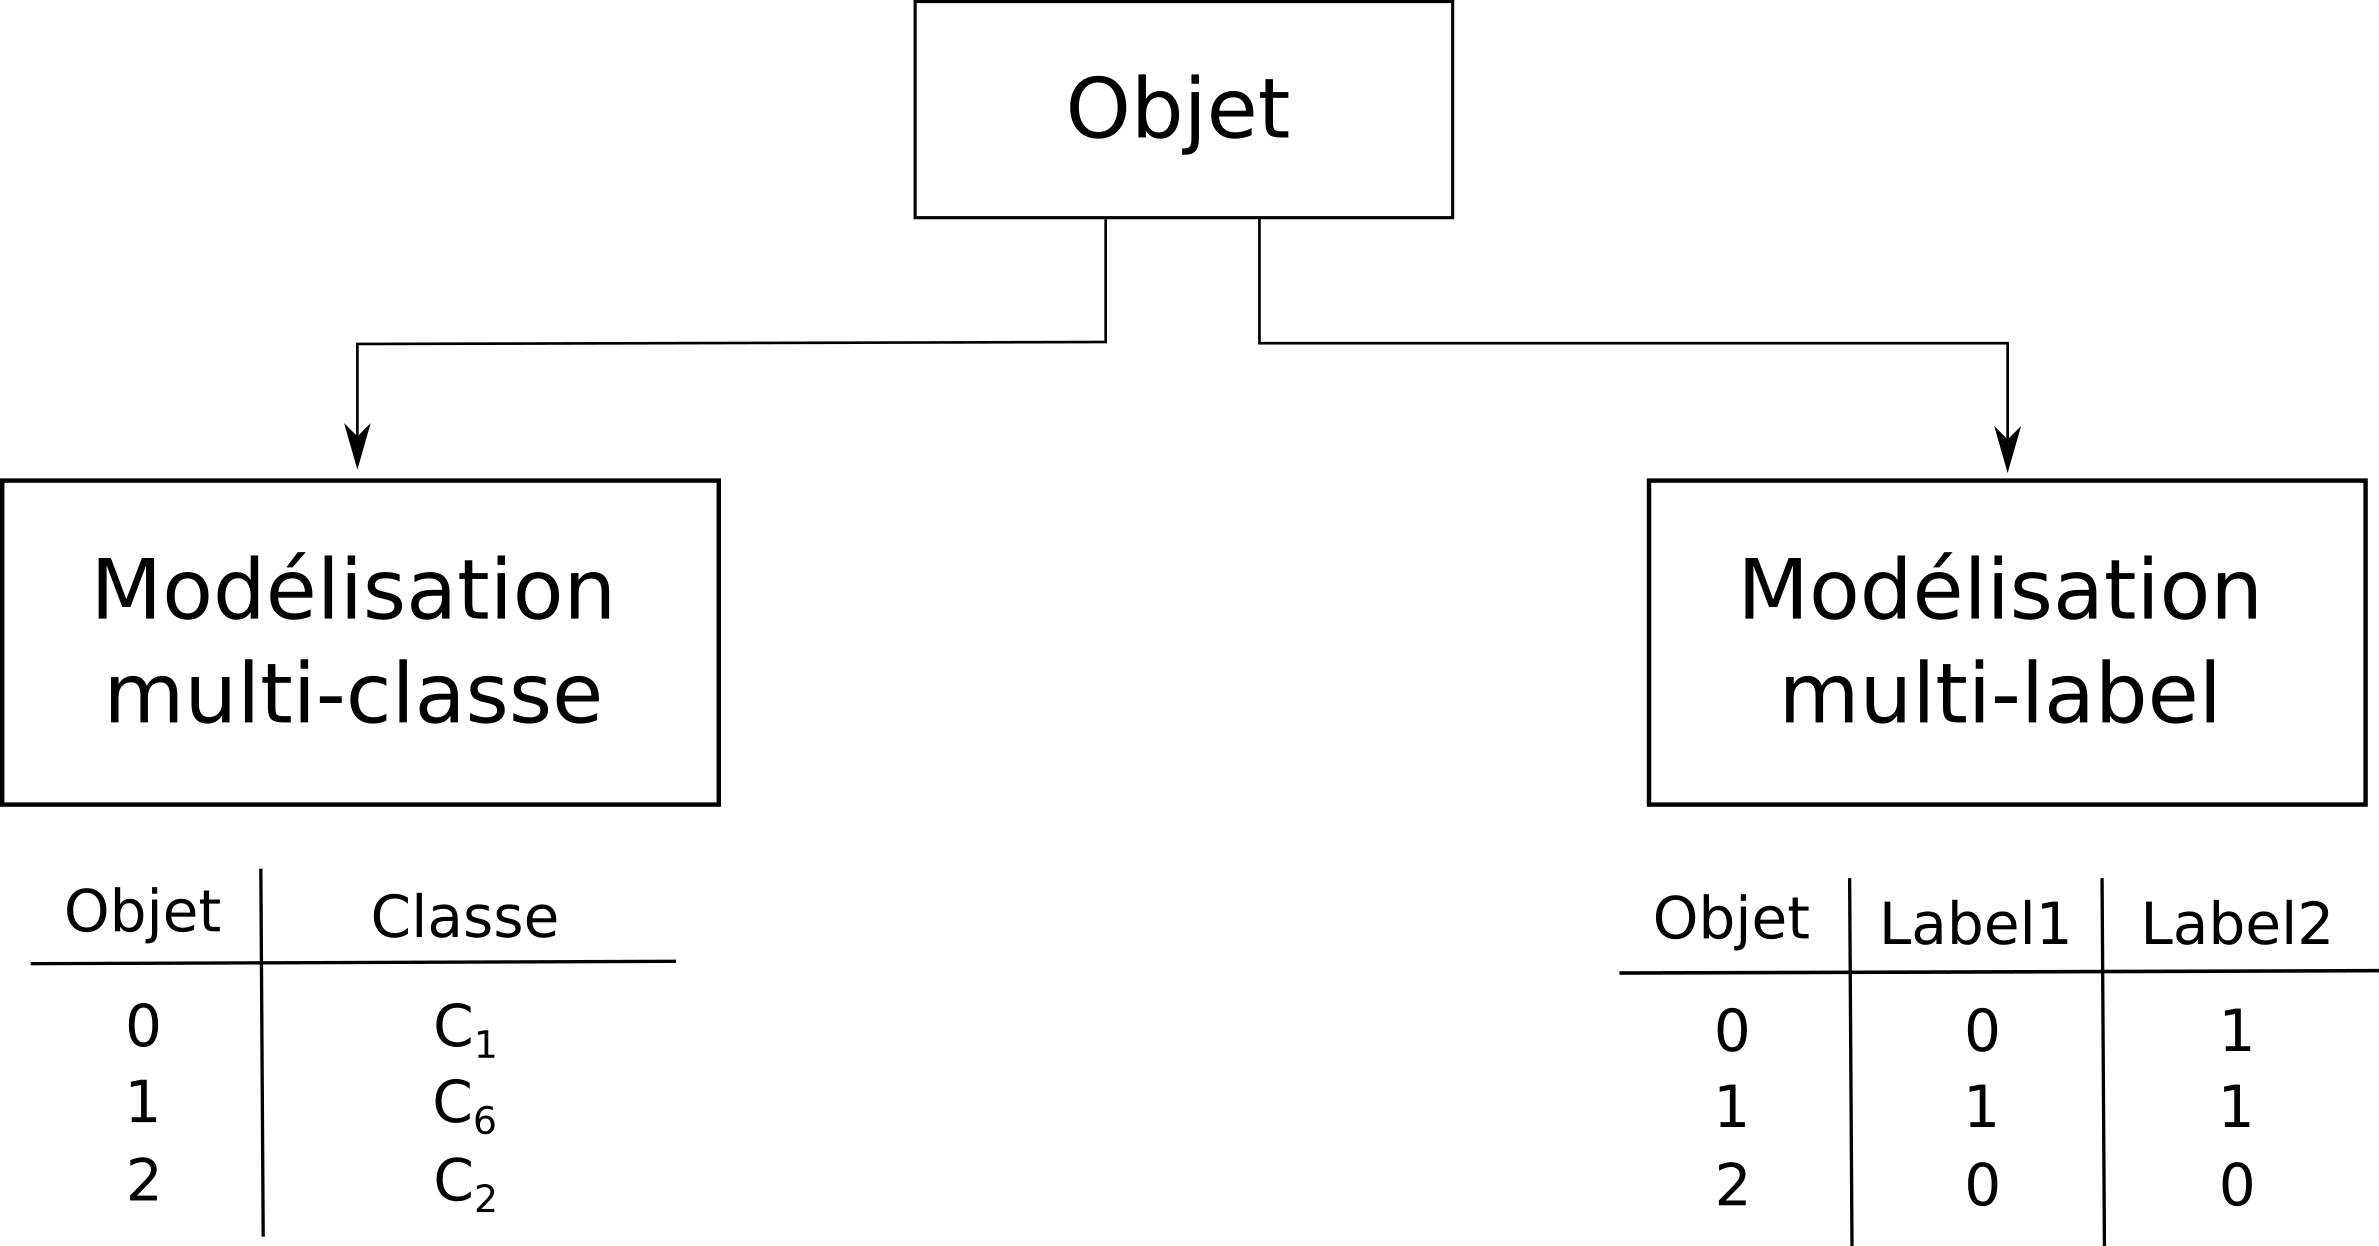
\includegraphics[scale=0.5]{modelisation.png}  \\
		\caption[Modélisation du problème]{Modélisation du problème}
		\label{fig:modelisation}
	\end{center}
\end{figure}

Le choix de la modélisation du problème a un impact sur le formalisme des données en entrée et en sortie du programme. Le choix de l’interface à montrer sera aussi déterminé par la modélisation. Ainsi, dans le cas multi-classe, un objet classifié ne sera lié qu’à une seule classe, ce qui impliquera de n’afficher que la classe concernée dans l’interface.\newline

Pour la première implémentation de l’interface, le modèle multi-classe a été privilégié pour faciliter la manipulation des données. Cependant, l’objectif est d’évoluer vers une modélisation multi-label du problème : l’interface programmée doit donc être flexible pour prendre en compte les différents formalismes. \newline

\section{Organisation des données}

\subsection{Données en entrée}

Dans une première modélisation du problème, on considère 4 jeux de données en entrée du programme :
\begin{itemize}[label=$\rightarrow$]
	\item \textbf{Un fichier « class.CSV »}, regroupant l’ensemble des classes d’erreur, suivies d’une brève description du type d’erreur.
	\item \textbf{Un fichier « results.CSV »}, regroupant les résultats de la phase de classification. On retrouve donc le numéro de l’entité, la classe qui lui est associée et une probabilité d’appartenance à cette classe.
	\item \textbf{Un dossier « emprise »}, regroupant les emprises des entités au format shapefile. L’identifiant de l’entité se retrouve dans le nom du fichier d'emprise (ex : « 2516.SHP » pour l’entité 2516).
	\item \textbf{Une orthoimage au format TIFF} de la zone analysée, spatialement superposable aux fichiers d’emprise au format .SHP.\newline
\end{itemize}


L’ensemble de ces données doit être fourni par l’utilisateur avant l’exécution du programme. Pour cela, une fenêtre de chargement des fichiers doit être implémentée. \newline

\textbf{Aperçu de la fenêtre de chargement}

\subsection{Données en sortie}

En sortie de l'interface, un seul fichier est retourné :
\begin{itemize}[label=$\rightarrow$]
	\item \textbf{Un fichier « modifyresults.CSV »}, regroupant les résultats de l'interaction avec l'utilisateur, sous une forme identique au fichier « results.CSV ». Deux méthodes sont envisageables : une première hypothèse consiste à sortir un tableau avec l'ensemble des entités testées (qu'elles soient modifiées ou non), et une seconde à ne restituer que les entités qui ont été modifiées.\newline
\end{itemize}

\textbf{Question : même si l'utilisateur confirme la classification, la probabilité est quand même modifiée et passe à 1 car on est sur de la classe ?! Il faudrait donc considérer toutes les entités traitées dans le fichier de sortie }

\subsection{Structuration des données}

\begin{itemize}
	\item Diagramme de classe
\end{itemize}



\section{Analyse fonctionnelle}

\subsection{Diagramme des cas d'utilisation (principales fonctionnalités à inclure)}

\subsection{Diagramme d'activité / détail des fonctions}

Détail des entrées et sorties / Description détaillée de la fonction (algo/pseudo-code/ADL) / Références en cas d'utilisation d'algorithmes existants\newline

\begin{itemize}
	\item Lecture des fichiers de classes (=> dictionnaire)
	\item Lecture des fichiers des résultats de la classification (=> matrice)
	\item Stratégies de choix des entités à présenter
	\begin{itemize}
		\item Plusieurs stratégies possibles
		\item Stratégies offline/online
	\end{itemize}
	\item Affichage
	\begin{itemize}
		\item Recherche des bâtiments dans les emprises
		\begin{itemize}
			\item si présence de l'identifiant = lancement du traitement
			\item sinon = popup d'erreur (flexibilité)
		\end{itemize}
		\item Lecture des fichiers .SHP
		\begin{itemize}
			\item calcul de la fenêtre d'affichage
			\item ajout des marges pour calculer les angles repères
		\end{itemize}
		\item Lecture de l'orthoimage
		\begin{itemize}
			\item recherche du point origine
			\item recherche de la taille d'un pixel
			\item calcul des coordonnées des angles de l'emprise en pixels dans l'orthoimage
			\item sélection de la matrice d'orthophoto correspondant et copie dans l'interface
		\end{itemize}
		\item Affichage de l'emprise
		\item Affichage du texte
		\begin{itemize}
			\item Affichage de l'entité en cours et de ses caractéristiques (classe actuelle et probabilité)
			\item Affichage des boutons de choix
		\end{itemize}
	\end{itemize}
	\item Interaction
	\begin{itemize}
		\item OK = passage à l'entité suivante
		\item pas OK
		\begin{itemize}
			\item affichage d'une fenêtre popup (différente selon le modèle)
			\item passage à l'entité suivante
		\end{itemize}
	\end{itemize}
\end{itemize}


\subsection{Conception de l'interface}

MVC

\subsection{Maquette du projet}




